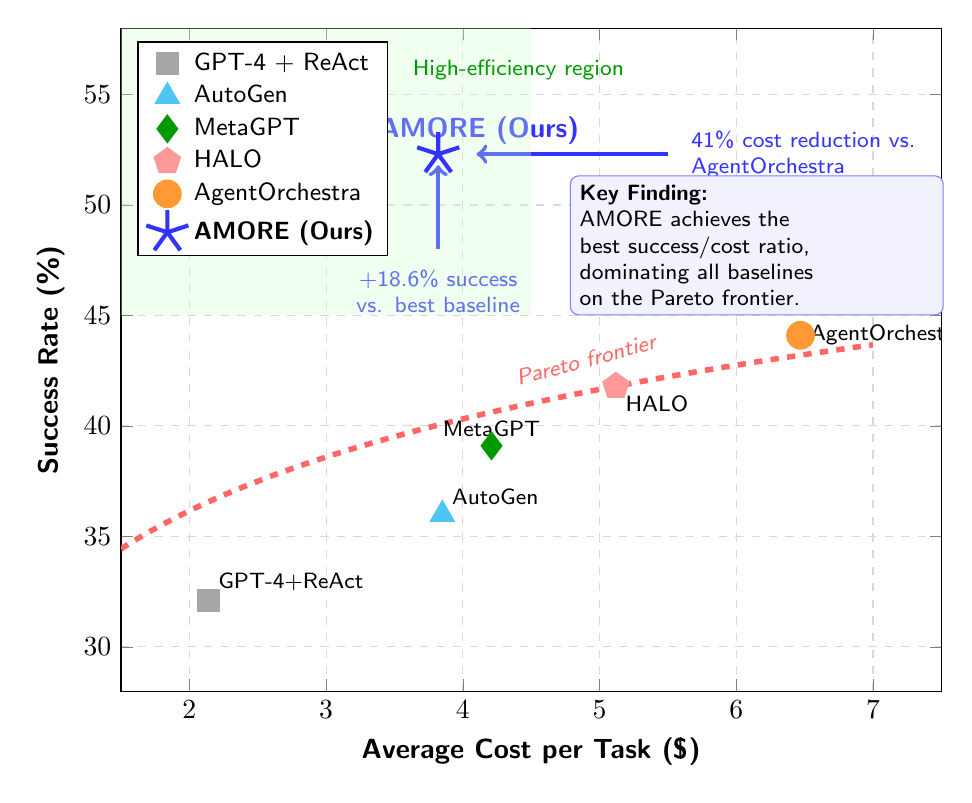
\begin{tikzpicture}
	\begin{axis}[
		width=12cm,
		height=10cm,
		xlabel={\textbf{Average Cost per Task (\$)}},
		ylabel={\textbf{Success Rate (\%)}},
		xmin=1.5,
		xmax=7.5,
		ymin=28,
		ymax=58,
		grid=both,
		grid style={dashed, gray!30},
		ylabel style={font=\sffamily\bfseries},
		xlabel style={font=\sffamily\bfseries},
		tick label style={font=\sffamily},
%		title={\sffamily\bfseries\large Cost-Performance Trade-off on MARS Benchmark},
		title style={yshift=8pt},
		legend style={
			at={(0.02,0.98)},
			anchor=north west,
			font=\sffamily\small,
			cells={anchor=west}
		}
		]
		% Scatter points for each method
		% GPT-4 + ReAct
		\addplot[
		only marks,
		mark=square*,
		mark size=4pt,
		color=gray!70
		] coordinates {(2.14, 32.1)};
		% AutoGen
		\addplot[
		only marks,
		mark=triangle*,
		mark size=5pt,
		color=cyan!70
		] coordinates {(3.85, 36.0)};
		% MetaGPT
		\addplot[
		only marks,
		mark=diamond*,
		mark size=5pt,
		color=green!60!black
		] coordinates {(4.21, 39.1)};
		% HALO
		\addplot[
		only marks,
		mark=pentagon*,
		mark size=5pt,
		color=pink!80!red
		] coordinates {(5.12, 41.8)};
		% AgentOrchestra
		\addplot[
		only marks,
		mark=otimes*,
		mark size=5pt,
		color=orange!80
		] coordinates {(6.47, 44.1)};
		% AMORE (Ours) - Highlighted with star
		\addplot[
		only marks,
		mark=star,
		mark size=8pt,
		color=blue!80,
		line width=1.5pt
		] coordinates {(3.82, 52.3)};
		% Pareto frontier (dashed line)
		\addplot[
		color=red!60,
		line width=2pt,
		dashed,
		domain=1.5:7,
		samples=100
		] {32 + 6*ln(x)};
		% Labels for each point
		\node[font=\sffamily\footnotesize, anchor=south west] at (axis cs:2.14,32.1) {GPT-4+ReAct};
		\node[font=\sffamily\footnotesize, anchor=south west] at (axis cs:3.85,36.0) {AutoGen};
		\node[font=\sffamily\footnotesize, anchor=south] at (axis cs:4.21,39.1) {MetaGPT};
		\node[font=\sffamily\footnotesize, anchor=north west] at (axis cs:5.12,41.8) {HALO};
		\node[font=\sffamily\footnotesize, anchor=west] at (axis cs:6.47,44.1) {AgentOrchestra};
		\node[font=\sffamily\bfseries, color=blue!80, anchor=south] at (axis cs:4.12,52.3) {\textbf{AMORE (Ours)}};
		% Annotation for AMORE's advantage
		\draw[->, line width=1.5pt, color=blue!80] (axis cs:5.5,52.3) -- (axis cs:4.1,52.3);
		\node[font=\sffamily\footnotesize, color=blue!80, anchor=west, text width=3cm] at (axis cs:5.6,52.3) {41\% cost reduction vs. AgentOrchestra};
		\draw[->, line width=1.5pt, color=blue!80] (axis cs:3.82,48) -- (axis cs:3.82,51.8);
		\node[font=\sffamily\footnotesize, color=blue!80, anchor=north, text width=2.5cm, align=center] at (axis cs:3.82,47.5) {+18.6\% success vs. best baseline};
		% Pareto frontier annotation
		\node[font=\sffamily\footnotesize\itshape, color=red!60, rotate=15] at (axis cs:4.9,43.0) {Pareto frontier};
		% Efficiency region annotation
		\fill[green!20, opacity=0.3] (axis cs:1.5,45) rectangle (axis cs:4.5,58);
		\node[font=\sffamily\footnotesize, color=green!60!black, anchor=north east] at (axis cs:5.25,57) {High-efficiency region};
		\legend{
			GPT-4 + ReAct,
			AutoGen,
			MetaGPT,
			HALO,
			AgentOrchestra,
			\textbf{AMORE (Ours)}
		}
	\end{axis}
	% Key insight box
	\node[draw=blue!50, fill=blue!5, rounded corners=3pt, font=\sffamily\footnotesize, text width=4.5cm, align=left, anchor=north west] at (5.7,6.55) {
		\textbf{Key Finding:}\\
		AMORE achieves the\\
		best success/cost ratio,\\
		dominating all baselines\\
		on the Pareto frontier.
	};
\end{tikzpicture}